\section{Swaptions As a Missing Link in Asset Allocation}
When constructing a portfolio, there are many considerations and therefore many choices. 
Some of the things we have to consider in asset allocation is deriversification, rebalancing 
and risk management. This Chapter will be a motivation of why it is important to be 
allocated to different asset classes. The purpose is to see in which market conditions
swaptions perform better compared to other asset classes.
\\\\
So a general  example is a 60/40 weight portfolio, where 60 percent is allocated to equities 
and 40 percent to fixed income. 
The investment belief in most portfolio is long beta, long duration, short volatility and short 
convexity. In other words the portfolio expectation is to earn a risk premium over the long term, 
where the asset have a long duration, to limit interest rate risk. And wanting to be short in
volatility, means willing to sell options to gain a risk premium. Secondly we will expect 
a short convexity portfolio to under perform when interest rate are volatile. 
\begin{figure}[H]
    \centering
    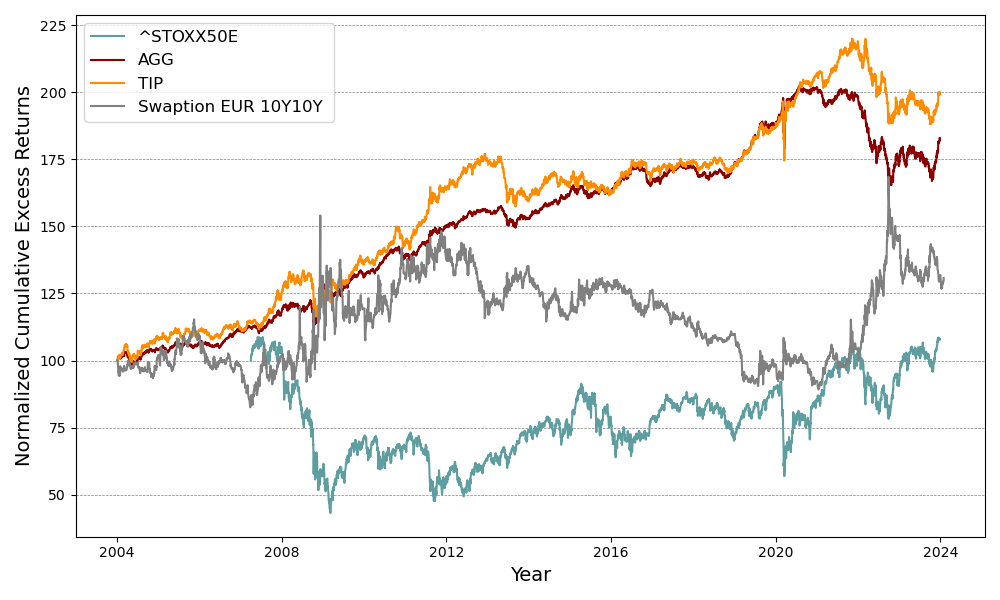
\includegraphics[scale = 0.4]{/Users/nannaingemannohrt/Desktop/master_thesis/main/plots/2004_to_2024_plot.png}
    \caption{Comparison of Normalized Cumulative Excess Return. Data source Citi Velocity 21.02.2024 
    and Yahoo Finance.}
    \label{fig:2004_2024}
\end{figure}
\noindent
Moving forward we will look at market data from Yahoo Finance and Citi Velocity. 
The purpose is to see how different asset classes perform under some particular markets situations.
First an introduction to the different tickers we will use to illustrate the different asset classes. 
We will like to compare perform of the asset classes equities, nominal bonds and inflation-linked bonds. 
The performance for the three asset classes will be compared to a swaption with ten years to expiry and a tenor
of ten years in euro, later in Chapter \ref{data_lab} the lingo of swaption will be covered. 
Below the chosen ticker are listed, with a short explanation. Where the ticker STOXX50E represent equities, 
AGG represent nominal bond and TIP illustrates inflation-linked bonds.

\begin{itemize}
    \item \textbf{STOXX50E} \text{---}  index of the 50 largest European equities.
    \item \textbf{AGG} \text{---}  index for US investment-grade bond. 
    \item \textbf{TIP} \text{---}  index for inflation-protected US-Treasury secitities.
    \end{itemize}
\noindent
Above in \autoref{fig:2004_2024} the three chosen ticker and the swaption development
is illustrated from 2004 to the start of 2024.
First of all we note that the same fluctuations appears across the three tickers. 
Secondly we note that these fluctuations does not appear in swaptions. 
We might even be able to see that the opposite fluctuation is present. 
Then lets remind yourself of some of the most important financial events during 
the time period from 2004 to 2024. First but not unnoticed we have the Global Financial Crisis
from 2007 to 2009.  Then we have the COVID-19 Pandemic in 2020 and most recently we have a 
longer period with high inflation starting i 2022. 
\\\\
To underline how swaption perform in these scenarios, we look a the specific time period
around some of the described events. Below in \autoref{fig:2007_2011} the same data is illustrated
from 2007 to 2011, this time period includes the Global Financial Crisis 2007 to 2009. 
From this time period we see that equities take a large jump down, where the development of the 
swaption was increasing. So during one of the worst drawdown period in the global market, 
swaptions kept performing. In \autoref{fig:2022_2024} we see the data displayed at the 
time period from 2022 to 2024, which is a period with high inflation. 
Here we clearly see that the swaption out perform the other asset classes. 
\\\\
This review on market data, underlines that swaption can add something different than some 
of the other asset classes. Therefore swaptions could add value to the portfolio constructions by adding diversification. 
But if swaptions should take part in the asset allocation, it is important to understand the instrument.
To understand swaptions as an instrument, we have to understand all the things contributing to the price
of a swaption. Then being able to price swaptions and analyzing them and managing the risk related to 
swaptions.  So moving forward we will start with a introduction to the mathematics of pricing swaptions. 
And troughout the thesis we will continue to develop knowledge of swaptions and the risk related to swaptions.
\begin{figure}[H]
    \centering
    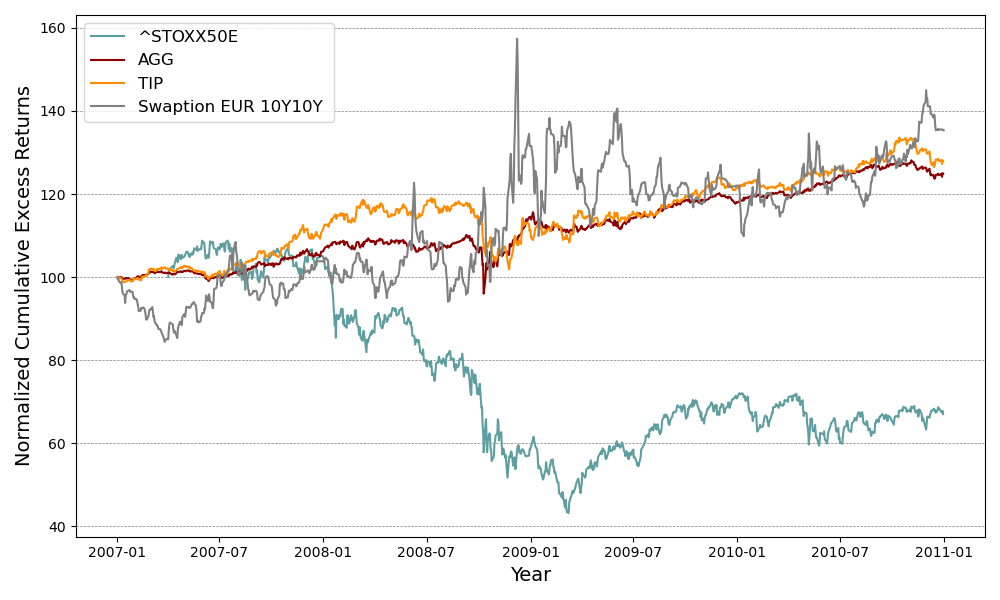
\includegraphics[scale = 0.4]{/Users/nannaingemannohrt/Desktop/master_thesis/main/plots/2007_to_2011.png}
    \caption{Global Financial Crisis 2007 to 2009.  Comparison of Normalized Cumulative Excess Return. Data source Citi Velocity 21.02.2024 
    and Yahoo Finance.}
    \label{fig:2007_2011}
\end{figure}
\noindent

\begin{figure}[H]
    \centering
    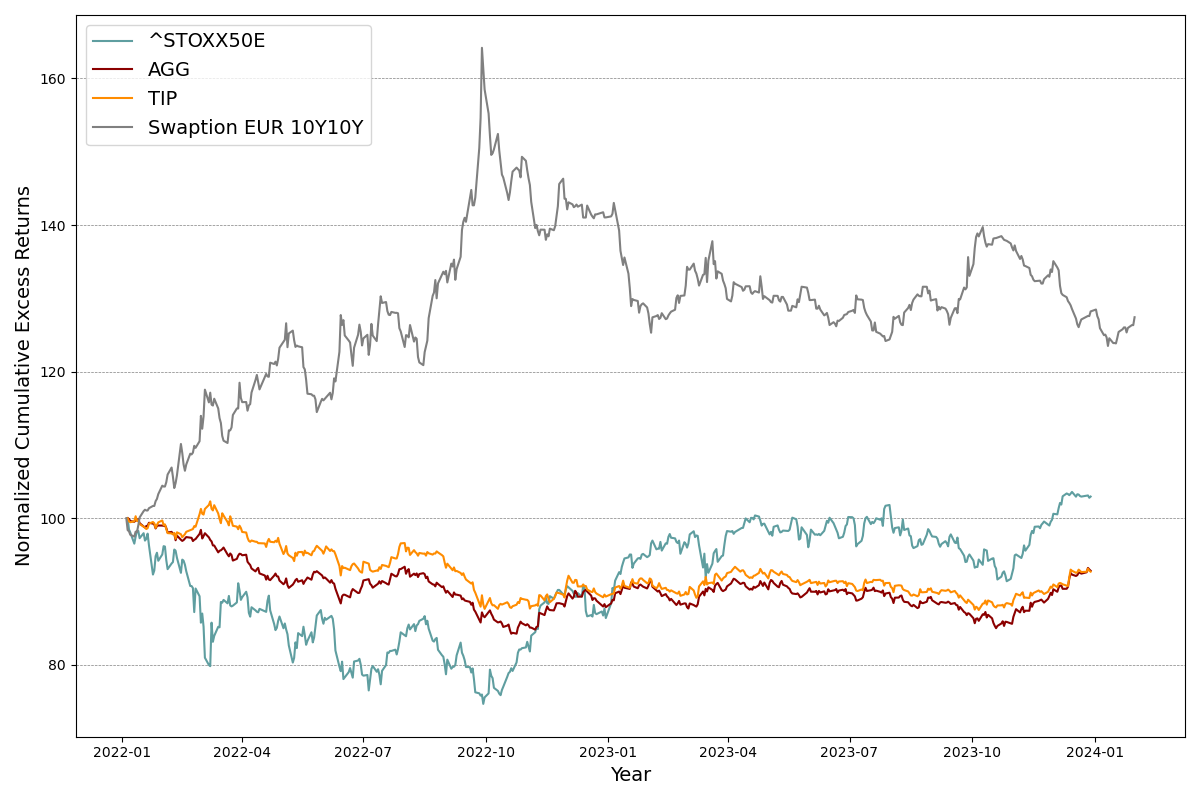
\includegraphics[scale = 0.4]{/Users/nannaingemannohrt/Desktop/master_thesis/main/plots/2022_to_2024.png}
    \caption{High inflation period 2022 to 2024. Comparison of Normalized Cumulative Excess Return. Data source Citi Velocity 21.02.2024 
    and Yahoo Finance.}
    \label{fig:2022_2024}
\end{figure}
\noindent

